%\maketitle

\tableofcontents

\newpage

\section{Задание}
\subsection{Условие}
По выданному преподавателем варианту разработать программу асинхронного обмена данными с внешним устройством. При помощи программы осуществить ввод или вывод информации, используя в качестве подтверждения данных сигнал (кнопку) готовности ВУ.

\begin{figure}[H]
\centering
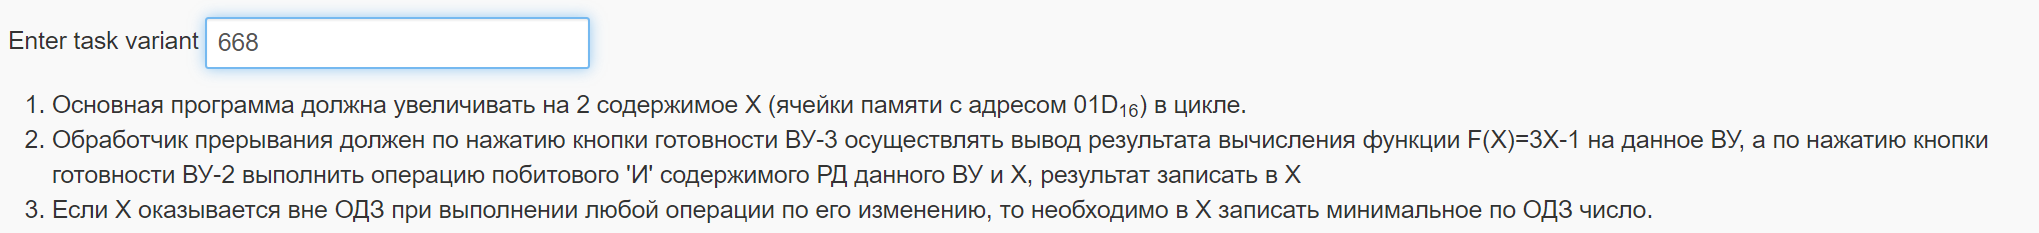
\includegraphics[scale=0.6]{task}
\label{pic:task}
\end{figure}

\subsection{Исходная строка}
Раздел планктонологии, занимающийся вопросами превращения неупорядоченной толпы идиотов в организованную, путем использования стадного инстинкта.
\subsection{Исходная строка в различных кодировках}
\noindent\resizebox{17.8cm}{!} {
	\begin{center}
		\begin{tabular}{|c|c|c|c||c|c|c|c||c|c|c|c||c|c|c|c|}
			\hline
			Символ & ISO-8859-5 & UTF-8 & UTF-16 & Символ & ISO-8859-5 & UTF-8 & UTF-16 & Символ & ISO-8859-5 & UTF-8 & UTF-16 & Символ & ISO-8859-5 & UTF-8 & UTF-16\\
			\hline
			\hline
			Р & C0 & D0 A0 & 04 20 & о & DE & D0 BE & 04 3E & т & E2 & D1 82 & 04 42 &   & 20 & 00 20 & 00 20\\
			а & D0 & D0 B0 & 04 30 & п & DF & D0 BF & 04 3F & о & DE & D0 BE & 04 3E & и & D8 & D0 B8 & 04 38\\
			з & D7 & D0 B7 & 04 37 & р & E0 & D1 80 & 04 40 & л & DB & D0 BB & 04 3B & с & E1 & D1 81 & 04 41\\
			д & D4 & D0 B4 & 04 34 & о & DE & D0 BE & 04 3E & п & DF & D0 BF & 04 3F & п & DF & D0 BF & 04 3F\\
			е & D5 & D0 B5 & 04 35 & с & E1 & D1 81 & 04 41 & ы & EB & D1 8B & 04 4B & о & DE & D0 BE & 04 3E\\
			л & DB & D0 BB & 04 3B & а & D0 & D0 B0 & 04 30 &   & 20 & 00 20 & 00 20 & л & DB & D0 BB & 04 3B\\
			& 20 & 00 20 & 00 20 & м & DC & D0 BC & 04 3C & и & D8 & D0 B8 & 04 38 & ь & EC & D1 8C & 04 4C\\
			п & DF & D0 BF & 04 3F & и & D8 & D0 B8 & 04 38 & д & D4 & D0 B4 & 04 34 & з & D7 & D0 B7 & 04 37\\
			л & DB & D0 BB & 04 3B &   & 20 & 00 20 & 00 20 & и & D8 & D0 B8 & 04 38 & о & DE & D0 BE & 04 3E\\
			а & D0 & D0 B0 & 04 30 & п & DF & D0 BF & 04 3F & о & DE & D0 BE & 04 3E & в & D2 & D0 B2 & 04 32\\
			н & DD & D0 BD & 04 3D & р & E0 & D1 80 & 04 40 & т & E2 & D1 82 & 04 42 & а & D0 & D0 B0 & 04 30\\
			к & DA & D0 BA & 04 3A & е & D5 & D0 B5 & 04 35 & о & DE & D0 BE & 04 3E & н & DD & D0 BD & 04 3D\\
			т & E2 & D1 82 & 04 42 & в & D2 & D0 B2 & 04 32 & в & D2 & D0 B2 & 04 32 & и & D8 & D0 B8 & 04 38\\
			о & DE & D0 BE & 04 3E & р & E0 & D1 80 & 04 40 &   & 20 & 00 20 & 00 20 & я & EF & D1 8F & 04 4F\\
			н & DD & D0 BD & 04 3D & а & D0 & D0 B0 & 04 30 & в & D2 & D0 B2 & 04 32 &   & 20 & 00 20 & 00 20\\
			о & DE & D0 BE & 04 3E & щ & E9 & D1 89 & 04 49 &   & 20 & 00 20 & 00 20 & с & E1 & D1 81 & 04 41\\
			л & DB & D0 BB & 04 3B & е & D5 & D0 B5 & 04 35 & о & DE & D0 BE & 04 3E & т & E2 & D1 82 & 04 42\\
			о & DE & D0 BE & 04 3E & н & DD & D0 BD & 04 3D & р & E0 & D1 80 & 04 40 & а & D0 & D0 B0 & 04 30\\
			г & D3 & D0 B3 & 04 33 & и & D8 & D0 B8 & 04 38 & г & D3 & D0 B3 & 04 33 & д & D4 & D0 B4 & 04 34\\
			и & D8 & D0 B8 & 04 38 & я & EF & D1 8F & 04 4F & а & D0 & D0 B0 & 04 30 & н & DD & D0 BD & 04 3D\\
			и & D8 & D0 B8 & 04 38 &   & 20 & 00 20 & 00 20 & н & DD & D0 BD & 04 3D & о & DE & D0 BE & 04 3E\\
			, & 2C & 00 2C & 00 2C & н & DD & D0 BD & 04 3D & и & D8 & D0 B8 & 04 38 & г & D3 & D0 B3 & 04 33\\
			& 20 & 00 20 & 00 20 & е & D5 & D0 B5 & 04 35 & з & D7 & D0 B7 & 04 37 & о & DE & D0 BE & 04 3E\\
			з & D7 & D0 B7 & 04 37 & у & E3 & D1 83 & 04 43 & о & DE & D0 BE & 04 3E &   & 20 & 00 20 & 00 20\\
			а & D0 & D0 B0 & 04 30 & п & DF & D0 BF & 04 3F & в & D2 & D0 B2 & 04 32 & и & D8 & D0 B8 & 04 38\\
			н & DD & D0 BD & 04 3D & о & DE & D0 BE & 04 3E & а & D0 & D0 B0 & 04 30 & н & DD & D0 BD & 04 3D\\
			и & D8 & D0 B8 & 04 38 & р & E0 & D1 80 & 04 40 & н & DD & D0 BD & 04 3D & с & E1 & D1 81 & 04 41\\
			м & DC & D0 BC & 04 3C & я & EF & D1 8F & 04 4F & н & DD & D0 BD & 04 3D & т & E2 & D1 82 & 04 42\\
			а & D0 & D0 B0 & 04 30 & д & D4 & D0 B4 & 04 34 & у & E3 & D1 83 & 04 43 & и & D8 & D0 B8 & 04 38\\
			ю & EE & D1 8E & 04 4E & о & DE & D0 BE & 04 3E & ю & EE & D1 8E & 04 4E & н & DD & D0 BD & 04 3D\\
			щ & E9 & D1 89 & 04 49 & ч & E7 & D1 87 & 04 47 & , & 2C & 00 2C & 00 2C & к & DA & D0 BA & 04 3A\\
			и & D8 & D0 B8 & 04 38 & е & D5 & D0 B5 & 04 35 &   & 20 & 00 20 & 00 20 & т & E2 & D1 82 & 04 42\\
			й & D9 & D0 B9 & 04 39 & н & DD & D0 BD & 04 3D & п & DF & D0 BF & 04 3F & а & D0 & D0 B0 & 04 30\\
			с & E1 & D1 81 & 04 41 & н & DD & D0 BD & 04 3D & у & E3 & D1 83 & 04 43 & . & 2E & 00 2E & 00 2E\\
			я & EF & D1 8F & 04 4F & о & DE & D0 BE & 04 3E & т & E2 & D1 82 & 04 42 &  &  &  & \\
			& 20 & 00 20 & 00 20 & й & D9 & D0 B9 & 04 39 & е & D5 & D0 B5 & 04 35 &  &  &  & \\
			в & D2 & D0 B2 & 04 32 &   & 20 & 00 20 & 00 20 & м & DC & D0 BC & 04 3C &  &  &  & \\
			\hline
		\end{tabular}
	\end{center}
}

\newpage
\section{Текст программы}
\subsection{Для ВУ-3}
\noindent\hspace*{2.5cm} ORG 0x516\\
ADDR: 	\hspace*{13mm}WORD \$STRING ; Адрес текущих двух символов\\
TMP\_LOOP:	\hspace*{3mm}WORD 0x2 ; Переменная, использующаяся для отделения одного символа от другого\\
\\
START: 	\hspace*{12mm}CLA ; Обеспечиваем реентерабельность\\
\hspace*{2.5cm} OUT 6\\
\\
BEGIN\_INIT:\hspace*{2mm}	LD \#0x2\\
\hspace*{2.5cm} ST TMP\_LOOP ; Для каждого элемента массива воссоздаем TMP\_LOOP\\
\\
BEGIN:\hspace*{13mm}	IN 7 ; Реализуем спин-луп для асинхронного вывода\\
\hspace*{2.5cm} AND \#0x40\\
\hspace*{2.5cm} BEQ BEGIN\\
\\
\hspace*{2.5cm} LOOP TMP\_LOOP\\
\hspace*{2.5cm} JUMP SMALL ; Обрабатываем младший байт\\
\hspace*{2.5cm} JUMP BIG ; Обрабатываем старший байт\\
\\
SMALL:	\hspace*{12mm}LD (ADDR)\\
\hspace*{2.5cm} PUSH\\
\hspace*{2.5cm} CALL \$CHECK\_SS ; Осуществляем проверку на стоп-символ\\
\hspace*{2.5cm} POP\\
\hspace*{2.5cm} OUT 6\\
\hspace*{2.5cm} JUMP BEGIN\\
\\
BIG:\hspace*{17mm}	LD (ADDR)+\\
\hspace*{2.5cm} SWAB\\
\hspace*{2.5cm} PUSH\\
\hspace*{2.5cm} CALL \$CHECK\_SS ; Осуществляем проверку на стоп-символ\\
\hspace*{2.5cm} POP\\
\hspace*{2.5cm} OUT 6\\
\hspace*{2.5cm} JUMP BEGIN\_INIT\\
\\
\\
STOP\_SYM:\hspace*{3mm}	WORD 0xD ; Стоп-символ\\
CHECK\_SS:\hspace*{3mm}	LD \&1 ; Подпрограмма для проверки на стоп-символ\\
\hspace*{2.5cm} SXTB\\
\hspace*{2.5cm} CMP STOP\_SYM\\
\hspace*{2.5cm} BEQ STOP\_PROG\\
\hspace*{2.5cm} RET\\
STOP\_PROG:\hspace*{1mm} HLT\\
\\
\\
\hspace*{2.4cm} ORG 0x59F\\
STRING: \hspace*{9mm}WORD 0xD0C0, 0xD4D7, 0xDBD5, 0xDF20, 0xD0DB, 0xDADD, 0xDEE2, 0xDEDD, 0xDEDB\\
\hspace*{25mm}WORD 0xD8D3, 0x2CD8, 0xD720, 0xDDD0, 0xDCD8, 0xEED0, 0xD8E9, 0xE1D9, 0x20EF\\
\hspace*{25mm}WORD 0xDED2, 0xE0DF, 0xE1DE, 0xDCD0, 0x20D8, 0xE0DF, 0xD2D5, 0xD0E0, 0xD5E9\\
\hspace*{25mm}WORD 0xD8DD, 0x20EF, 0xD5DD, 0xDFE3, 0xE0DE, 0xD4EF, 0xE7DE, 0xDDD5, 0xDEDD\\
\hspace*{25mm}WORD 0x20D9, 0xDEE2, 0xDFDB, 0x20EB, 0xD4D8, 0xDED8, 0xDEE2, 0x20D2, 0x20D2\\
\hspace*{25mm}WORD 0xE0DE, 0xD0D3, 0xD8DD, 0xDED7, 0xD0D2, 0xDDDD, 0xEEE3, 0x202C, 0xE3DF\\
\hspace*{25mm}WORD 0xD5E2, 0x20DC, 0xE1D8, 0xDEDF, 0xECDB, 0xDED7, 0xD0D2, 0xD8DD, 0x20EF\\
\hspace*{25mm}WORD 0xE2E1, 0xD4D0, 0xDEDD, 0xDED3, 0xD820, 0xE1DD, 0xD8E2, 0xDADD, 0xD0E2\\
\hspace*{25mm}WORD 0x0D2E\\

%\newpage
%\subsection{Для ВУ-5}
%\noindent\hspace*{2.5cm} ORG 0x516\\
%ADDR: 	\hspace*{13mm}WORD \$STRING ; Адрес текущих двух символов\\
%TMP\_LOOP:	\hspace*{3mm}WORD 0x2 ; Переменная, использующаяся для отделения одного символа от другого\\
%\\
%START: 	\hspace*{12mm}CLA ; Обеспечиваем реентерабельность\\
%\hspace*{2.5cm} OUT 6\\
%\\
%BEGIN\_INIT:\hspace*{2mm}	LD \#0x2\\
%\hspace*{2.5cm} ST TMP\_LOOP ; Для каждого элемента массива воссоздаем TMP\_LOOP\\
%\\
%BEGIN:\hspace*{13mm} LOOP TMP\_LOOP\\
%\hspace*{2.5cm} JUMP SMALL ; Обрабатываем младший байт\\
%\hspace*{2.5cm} JUMP BIG ; Обрабатываем старший байт\\
%\\
%SMALL:	\hspace*{12mm}LD (ADDR)\\
%\hspace*{2.5cm} PUSH\\
%\hspace*{2.5cm} CALL \$CHECK\_SS ; Осуществляем проверку на стоп-символ\\
%\hspace*{2.5cm} POP\\
%\hspace*{2.5cm} OUT 0xC\\
%\hspace*{2.5cm} JUMP BEGIN\\
%\\
%BIG:\hspace*{17mm}	LD (ADDR)+\\
%\hspace*{2.5cm} SWAB\\
%\hspace*{2.5cm} PUSH\\
%\hspace*{2.5cm} CALL \$CHECK\_SS ; Осуществляем проверку на стоп-символ\\
%\hspace*{2.5cm} POP\\
%\hspace*{2.5cm} OUT 0xC\\
%\hspace*{2.5cm} JUMP BEGIN\_INIT\\
%\\
%\\
%STOP\_SYM:\hspace*{3mm}	WORD 0xD ; Стоп-символ\\
%CHECK\_SS:\hspace*{3mm}	LD \&1 ; Подпрограмма для проверки на стоп-символ\\
%\hspace*{2.5cm} SXTB\\
%\hspace*{2.5cm} CMP STOP\_SYM\\
%\hspace*{2.5cm} BEQ STOP\_PROG\\
%\hspace*{2.5cm} RET\\
%STOP\_PROG:\hspace*{1mm} HLT\\
%\\
%\\
%\hspace*{2.4cm} ORG 0x59F\\
%STRING: \hspace*{9mm}WORD 0xD0C0, 0xD4D7, 0xDBD5, 0xDF20, 0xD0DB, 0xDADD, 0xDEE2, 0xDEDD, 0xDEDB\\
%\hspace*{25mm}WORD 0xD8D3, 0x2CD8, 0xD720, 0xDDD0, 0xDCD8, 0xEED0, 0xD8E9, 0xE1D9, 0x20EF\\
%\hspace*{25mm}WORD 0xDED2, 0xE0DF, 0xE1DE, 0xDCD0, 0x20D8, 0xE0DF, 0xD2D5, 0xD0E0, 0xD5E9\\
%\hspace*{25mm}WORD 0xD8DD, 0x20EF, 0xD5DD, 0xDFE3, 0xE0DE, 0xD4EF, 0xE7DE, 0xDDD5, 0xDEDD\\
%\hspace*{25mm}WORD 0x20D9, 0xDEE2, 0xDFDB, 0x20EB, 0xD4D8, 0xDED8, 0xDEE2, 0x20D2, 0x20D2\\
%\hspace*{25mm}WORD 0xE0DE, 0xD0D3, 0xD8DD, 0xDED7, 0xD0D2, 0xDDDD, 0xEEE3, 0x202C, 0xE3DF\\
%\hspace*{25mm}WORD 0xD5E2, 0x20DC, 0xE1D8, 0xDEDF, 0xECDB, 0xDED7, 0xD0D2, 0xD8DD, 0x20EF\\
%\hspace*{25mm}WORD 0xE2E1, 0xD4D0, 0xDEDD, 0xDED3, 0xD820, 0xE1DD, 0xD8E2, 0xDADD, 0xD0E2\\
%\hspace*{25mm}WORD 0x0D2E\\

\newpage

\section{Описание программы}
\subsection{Назначение программы}
Асинхронный посимвольный вывод заранее заданой строки в кодировке ISO-8859-5 на ВУ-3. По условию задания строка хранится в памяти в виде массива, начиная с ячейки 59F. При чем в каждом элементе хранится по два символа. Цикл вывода символов оканчивается по символу 0D.

\subsection{Область представления и область допустимых значений исходных данных и результата}
\subsubsection{Область представления}
 ADDR - 11-разрядное беззнаковое число с фиксированной запятой. Диапазон значений формата $ 0\ldots2^{11}-1 $\\
\\
Ячейки, содержащие символы строки - 16-разрядные беззнаковые числа с фиксированной запятой. Диапазон значений формата $ 0\ldots2^{16}-1 $\\

\subsubsection{Область допустимых значений}
\noindent Область допустимых значений ADDR (для первого элемента массива):
\[
	\begin{cases}
		[0, 516 - L_{16}]\cup[536, 800] & \text{, при L: [0, 516]}\\
		[536, 800 - (L_{16} - 516)] & \text{, при L: [517, 777]}\\
	\end{cases}
\] 
где $ L_{16} $ - длина массива, в котором организовано хранение символов. Рассчитывается как: \[
L_{10} = \begin{cases}
		\frac{l}{2} + 1, & \text{если l - четное}\\
		\frac{l}{2} + 0,5, & \text{если l - нечетное}\\
\end{cases}
\]\\
где $ l $ - длина строки.\\
\\
Длина вводимой строки для заданного по заданию ADDR: $ [0, EEE] $

\subsection{Расположение в памяти ЭВМ программы, исходных данных и результатов}
\subsubsection{Исходные данные и результат}
\noindent ADDR (516) - содержит адрес текущего обрабатываемого элемента массива. В самом начале указывает на первый элемент массива.\\
\\
STRING (59F) - содержит первый элемент массива

\subsubsection{Программа}
\noindent 518 - 52E - основная программа\\
530 - 535 - подпрограмма по проверке на стоп-символ\\
517 - переменная, используемая в основной программе\\
52F - константа, используемая подпрограммой\\
$59F\ldots 59F + (L - 1)$ - расположение в памяти строки (L - длина массива, вычисляется в 3.2.2)

\subsection{Адреса первой и последней исполняемой команд.}
\noindent 518 - первая исполняемая команда программы\\
535 - последняя исполняемая команда программы

\newpage

\section{Таблица трассировки}
\begin{center}
	\begin{tabular}{|c|c|c|c|c|c|c|c|c|c|c|c|}
		\hline
		\multicolumn{2}{|c}{\makecell{\textbf{Выполняемая}\\\textbf{команда}}}
		&\multicolumn{8}{|c|}{\textbf{Содердимое регистров после выполнения команды}}
		&\multicolumn{2}{c|}{\makecell{\textbf{Ячейка, содержимое}\\\textbf{которой изменилось}}}\\
		\hline
		Адрес & Код & IP & CR & AR & DR & SP & BR & AC & NZVC & Адрес & Новый код\\
		\hline
		518 & 0200 & 519 & 0200 & 518 & 0200 & 000 & 0518 & 0000 & 0100 &  & \\
		519 & 1306 & 51A & 1306 & 519 & 1306 & 000 & 0519 & 0000 & 0100 &  & \\
		\hline
		51A & AF02 & 51B & AF02 & 51A & 0002 & 000 & 0002 & 0002 & 0000 &  & \\
		51B & EEFB & 51C & EEFB & 517 & 0002 & 000 & FFFB & 0002 & 0000 & 517 & 0002\\
		\hline
		51C & 1207 & 51D & 1207 & 51C & 1207 & 000 & 051C & 0040 & 0000 &  & \\
		51D & 2F40 & 51E & 2F40 & 51D & 0040 & 000 & 0040 & 0040 & 0000 &  & \\
		51E & F0FD & 51F & F0FD & 51E & F0FD & 000 & 051E & 0040 & 0000 &  & \\
		51F & 8EF7 & 520 & 8EF7 & 517 & 0001 & 000 & 0000 & 0040 & 0000 &  & \\
		520 & CE01 & 522 & CE01 & 520 & 0522 & 000 & 0001 & 0040 & 0000 &  & \\
		522 & A8F3 & 523 & A8F3 & 59F & D0C0 & 000 & FFF3 & D0C0 & 1000 &  & \\
		523 & 0C00 & 524 & 0C00 & 7FF & D0C0 & 7FF & 0523 & D0C0 & 1000 &  & \\
		524 & D530 & 530 & D530 & 7FE & 0525 & 7FE & D530 & D0C0 & 1000 &  & \\
		530 & AC01 & 531 & AC01 & 7FF & D0C0 & 7FE & 0001 & D0C0 & 1000 &  & \\
		531 & 0600 & 532 & 0600 & 531 & 0600 & 7FE & 0531 & FFC0 & 1000 &  & \\
		532 & 7EFC & 533 & 7EFC & 52F & 000D & 7FE & FFFC & FFC0 & 1001 &  & \\
		533 & F001 & 534 & F001 & 533 & F001 & 7FE & 0533 & FFC0 & 1001 &  & \\
		534 & 0A00 & 525 & 0A00 & 7FE & 0525 & 7FF & 0534 & FFC0 & 1001 &  & \\
		525 & 0800 & 526 & 0800 & 7FF & D0C0 & 000 & 0525 & D0C0 & 1001 &  & \\
		526 & 1306 & 527 & 1306 & 526 & 1306 & 000 & 0526 & D0C0 & 1001 &  & \\
		527 & CEF4 & 51C & CEF4 & 527 & 051C & 000 & FFF4 & D0C0 & 1001 &  & \\
		\hline
		51C & 1207 & 51D & 1207 & 51C & 1207 & 000 & 051C & D000 & 1001 &  & \\
		51D & 2F40 & 51E & 2F40 & 51D & 0040 & 000 & 0040 & 0000 & 0101 &  & \\
		51E & F0FD & 51C & F0FD & 51E & F0FD & 000 & FFFD & 0000 & 0101 &  & \\
		\hline
		51C & 1207 & 51D & 1207 & 51C & 1207 & 000 & 051C & 0040 & 0101 &  & \\
		51D & 2F40 & 51E & 2F40 & 51D & 0040 & 000 & 0040 & 0040 & 0001 &  & \\
		51E & F0FD & 51F & F0FD & 51E & F0FD & 000 & FFFD & 0040 & 0001 &  & \\
		51F & 8EF7 & 521 & 8EF7 & 517 & 0000 & 000 & FFFF & 0040 & 0001 &  & \\
		521 & CE06 & 528 & CE06 & 521 & 0528 & 000 & 0006 & 0040 & 0001 &  & \\
		528 & AAED & 529 & AAED & 59F & D0C0 & 000 & FFED & D0C0 & 1001 &  & \\
		529 & 0680 & 52A & 0680 & 529 & 0680 & 000 & 0529 & C0D0 & 1001 &  & \\
		52A & 0C00 & 52B & 0C00 & 7FF & C0D0 & 7FF & 052A & C0D0 & 1001 &  & \\
		52B & D530 & 530 & D530 & 7FE & 052C & 7FE & D530 & C0D0 & 1001 &  & \\
		530 & AC01 & 531 & AC01 & 7FF & C0D0 & 7FE & 0001 & C0D0 & 1001 &  & \\
		531 & 0600 & 532 & 0600 & 531 & 0600 & 7FE & 0531 & FFD0 & 1001 &  & \\
		532 & 7EFC & 533 & 7EFC & 52F & 000D & 7FE & FFFC & FFD0 & 1001 &  & \\
		533 & F001 & 534 & F001 & 533 & F001 & 7FE & 0533 & FFD0 & 1001 &  & \\
		534 & 0A00 & 52C & 0A00 & 7FE & 052C & 7FF & 0534 & FFD0 & 1001 &  & \\
		52C & 0800 & 52D & 0800 & 7FF & C0D0 & 000 & 052C & C0D0 & 1001 &  & \\
		52D & 1306 & 52E & 1306 & 52D & 1306 & 000 & 052D & C0D0 & 1001 &  & \\
		52E & CEEB & 51A & CEEB & 52E & 051A & 000 & FFEB & C0D0 & 1001 &  & \\
		\hline
		
	\end{tabular}
\end{center}
\newpage

\section{Вывод}
В ходе выполнения лабораторной работы я разобрался как работают команды, связанные с организацией ввода-вывода. Научился писать простые программы на ассемблере БЭВМ.
